\documentclass{worksheet}

\usepackage{svg}
\usepackage{nicematrix}
\usepackage{tikz}
\usepackage{multicol}
\usepackage{tcolorbox}
\usetikzlibrary{shapes.geometric, positioning}



\title{Stochastic Environments Practice}
\author{CIS 5210}
\date{March 18, 2025}

\begin{document}

\maketitle


\begin{question}[Expectimax][]

What is the expected utility of picking action $a_1$? What is the expected utility of picking action $a_2$? Using Expectimax, which action will the Max player select? \textit{(You might need a calculator.)}

\begin{center}
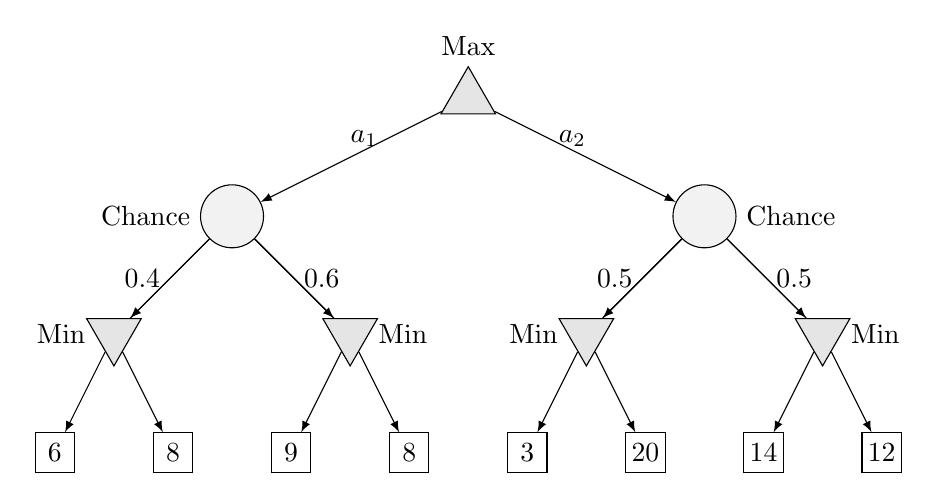
\begin{tikzpicture}[
    % Define node styles
    max/.style={
        regular polygon,
        regular polygon sides=3,  % Triangle
        draw,
        fill=gray!20,
        minimum size=0.8cm,
        inner sep=0pt
    },
    min/.style={
        regular polygon,
        regular polygon sides=3,  % Triangle
        draw,
        fill=gray!20,
        shape border rotate=180,  % Rotates the triangle to point down
        minimum size=0.8cm,
        inner sep=0pt
    },
    chance/.style={
        circle,
        draw,
        fill=gray!10,
        minimum size=0.8cm,
        inner sep=0pt
    },
    leaf/.style={
        rectangle,
        draw,
        minimum width=0.5cm,
        minimum height=0.5cm,
        inner sep=2pt
    },
    level 1/.style={sibling distance=6cm},
    level 2/.style={sibling distance=3cm},
    level 3/.style={sibling distance=1.5cm},
    edge from parent/.style={draw, -latex}
]
    % Root node (MAX)
    \node[max, label=above:{Max}] (root) {}
        % First level - Chance nodes
        child {
            node[chance, label=left:{Chance}] (c1) {}
            % Second level from c1 - MIN nodes
            child {
                node[min, label=left:{Min}] (m1) {}
                % Third level from m1 - leaf nodes
                child { node[leaf] {6} }
                child { node[leaf] {8} }
            }
            child {
                node[min, label=right:{Min}] (m2) {}
                % Third level from m2 - leaf nodes
                child { node[leaf] {9} }
                child { node[leaf] {8} }
            }
            % Edge labels
            edge from parent node[left, pos=0.3] {$a_1$}
        }
        child {
            node[chance, label=right:{Chance}] (c2) {}
            % Second level from c2 - MIN nodes
            child {
                node[min, label=left:{Min}] (m3) {}
                % Third level from m3 - leaf nodes
                child { node[leaf] {3} }
                child { node[leaf] {20} }
            }
            child {
                node[min, label=right:{Min}] (m4) {}
                % Third level from m4 - leaf nodes
                child { node[leaf] {14} }
                child { node[leaf] {12} }
            }
            % Edge labels
            edge from parent node[right, pos=0.3] {$a_2$}
        };
        
    % Add probability labels to the chance nodes' children
    \draw (c1) -- (m1) node[midway, left] {0.4};
    \draw (c1) -- (m2) node[midway, right] {0.6};
    \draw (c2) -- (m3) node[midway, left] {0.5};
    \draw (c2) -- (m4) node[midway, right] {0.5};
\end{tikzpicture}
\end{center}    

\end{question}

% \shortanswerspace

% \begin{solution}

% Expected utility of $a_1$ is $0.4 * 6 + 0.6 * 8 = 7.2$.
% Expected utility of $a_2$ is $0.5 * 3 + 0.5 * 12 = 7.5$.
% Max will play $a_2$.
% \end{solution}


\begin{question}[Signal in the Noise][]
Consider a grid-based agent in a Markov Decision Process setting. In these settings, we assume that the agent moves in the direction specified by their action with a certain probability. If the agent does not move in the intended direction, they choose uniformly at random from one of the two directions offset by 90 degrees from the intended direction. (Intending to move LEFT, the agent might move LEFT, UP, or DOWN, but never RIGHT.) The probability that an agent moves in the wrong direction is referred to as the \textit{noise value}.

If an agent has a noise value of $0.2$, fill in the blanks in the terms below representing the agent's transition function for taking the action UP from the state represented by coordinate $(x=5, y=5)$ with no adjacent obstacles or boundaries. Higher coordinates are to the right and up.

\begin{itemize}
    \item $T((5, 5), \text{UP}, (5, 5)) = $ \_\_\_\_\_
    \item $T((5, 5), \text{UP}, (4, 5)) = $ \_\_\_\_\_
    \item $T((5, 5), \text{UP}, (6, 5)) = $ \_\_\_\_\_
    \item $T((5, 5), \text{UP}, (5, 4)) = $ \_\_\_\_\_
    \item $T((5, 5), \text{UP}, (5, 6)) = $ \_\_\_\_\_
\end{itemize}
    
\end{question}

% \begin{solution}

% \begin{itemize}
%     \item $T((5, 5), \text{UP}, (5, 5)) = 0$ 
%     \item $T((5, 5), \text{UP}, (4, 5)) = 0.1$ 
%     \item $T((5, 5), \text{UP}, (6, 5)) = 0.1$ 
%     \item $T((5, 5), \text{UP}, (5, 4)) = 0$ 
%     \item $T((5, 5), \text{UP}, (5, 6)) = 0.8$ 
% \end{itemize}

% \end{solution}

\pagebreak

\begin{question}
The Hyperdrive MDP is described by the following transition and reward functions:

\begin{center}
\begin{tabular}{c|ccc}
$T(s, a, s')$ & Cruising & Hyperspace & Crashed \\
\hline
Cruising, Maintain & $1.0$ & $0$ & $0$ \\
Cruising, Punch It & $0.5$ & $0.5$ & $0$ \\
Hyperspace, Maintain & $0.5$ & $0.5$ & $0$ \\
Hyperspace, Punch It & $0$ & $0$ & $1.0$ \\
Crashed, $*$ & $0$ & $0$ & $1.0$ \\
\end{tabular}
\end{center}

\begin{center}
\begin{tabular}{c|ccc}
$R(s, a, s')$ & Cruising & Hyperspace & Crashed \\
\hline
Cruising, Maintain & $1$ & $1$ & $0$ \\
Cruising, Punch It & $2$ & $2$ & $0$ \\
Hyperspace, Maintain & $1$ & $1$ & $0$ \\
Hyperspace, Punch It & $0$ & $0$ & $-10$ \\
Crashed, $*$ & $0$ & $0$ & $0$ \\
\end{tabular}
\end{center}

\begin{enumerate}
    \item Assume that the start state is always ``Cruising". Come up with two policies $\pi_1$ and $\pi_2$ that lead to guaranteed infinite rewards in a setting of the game where the horizon is infinite and $\gamma = 1.0$.
    \item If the setting is changed so that $0 < \gamma < 1$, the values of each state will converge to a finite value after a certain number of actions. Can you modify the game in a different way, without changing $\gamma$, so that the values would also converge to a finite value? As a hint, consider the role of ``Crashed" as an \textit{absorbing state}.
\end{enumerate}

\end{question}

% \begin{solution}

% \begin{enumerate}
%     \item $\pi_1(s) = $ Maintain for all values of $s$. $\pi_2(\text{Cruising}) = $ Punch It, $\pi_2(\text{Hyperspace}) = $ Maintain
%     \item Adjust the probabilities so that ``Crashed" is reachable from all actions and all states. In the limit, a player will crash, capping expected utility. 
% \end{enumerate}

% \end{solution}

\end{document}